\documentclass[8pt]{beamer} % dvipsnames gives more built-in colors
\usepackage{graphicx}

\usetheme{Madrid}
\useoutertheme{miniframes} % Alternatively: miniframes, infolines, split
\useinnertheme{circles}

\definecolor{UBCblue}{rgb}{0.04706, 0.13725, 0.26667} % UBC Blue (primary)

\usecolortheme[named=UBCblue]{structure}
%\usecolortheme[named=Mahogany]{structure} % Sample dvipsnames color



\title{Paper Review - Auto-FuzzyJoin: Auto-Program Fuzzy Similarity Joins Without Labelled Examples}
\subtitle{Peng Li, Xiang Cheng, Xu Chu, Yeye He, Surajit Chaudhuri}
\date{\today}
\author{Carmel Gafa}


\begin{document}

\setbeamercolor{myblock}{bg=red!10, fg=black}

\begin{frame}[plain]
    \maketitle
\end{frame}


\begin{frame}{Fuzzy-join (or similarity join)}
	\begin{figure}
		\centering
		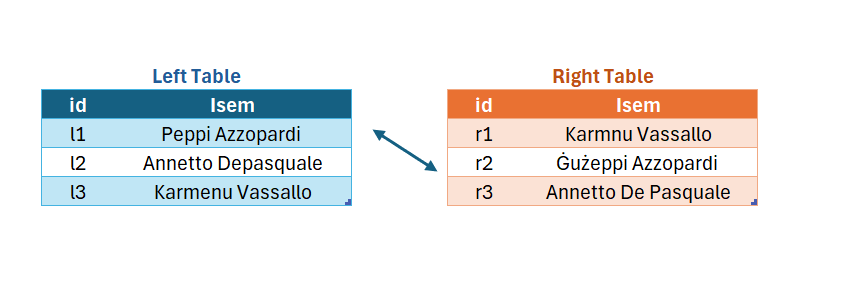
\includegraphics[width=0.7\linewidth]{FuzzyJoin}
	\end{figure}

	\begin{figure}
		\centering
		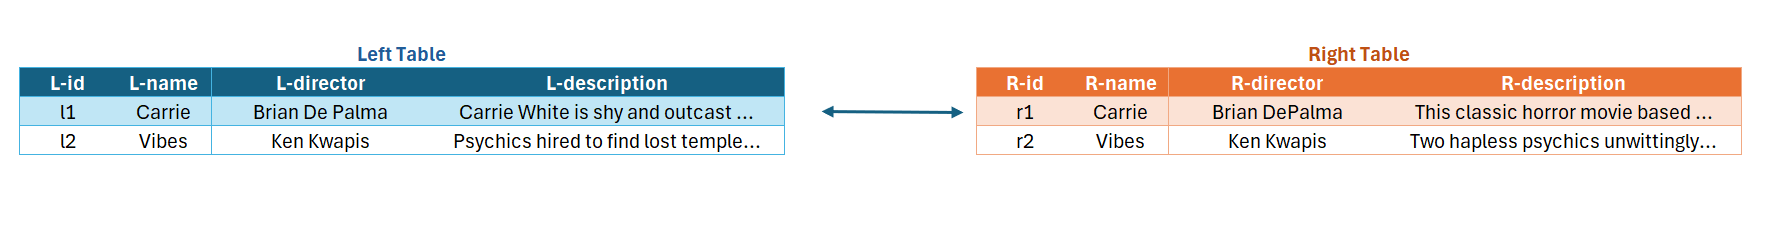
\includegraphics[width=1\linewidth]{img/FuzzyJoin_2}
	\end{figure}

	\begin{itemize}
		\item Fuzzy join takes two tables as inputs and identify record pairs that refer to the same entity
		\item As an example, l1 and r2 refer to the same person
		\item The concept can be extended to rows consisting of multiple columns
	\end{itemize}
\end{frame}




\begin{frame}{Fuzzy-join configuration }
 \begin{tabular}{ccc}  
	\begin{tabular}{c}
		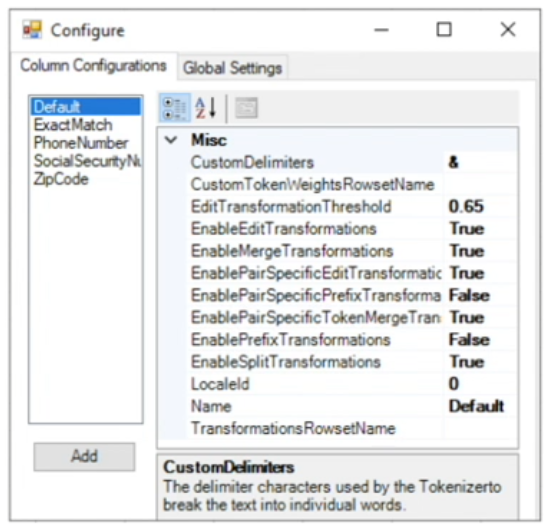
\includegraphics[width=0.2\linewidth]{img/FuzzyJoin_config_1.png}
	\end{tabular}
	& \begin{tabular}{l}
		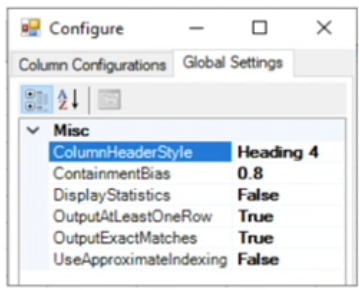
\includegraphics[width=0.2\linewidth]{img/FuzzyJoin_config_2.png}
	\end{tabular}	
	& \begin{tabular}{l}
	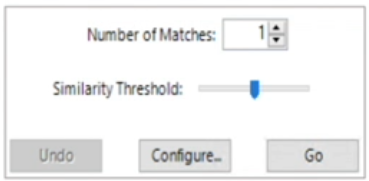
\includegraphics[width=0.2\linewidth]{img/FuzzyJoin_config_3.png}
	\end{tabular}  \\
\end{tabular}

\begin{itemize}
	\item Fuzzy-join has been integrated many commercial applications
	\item These systems are normally not easy to use as they have a big number of configuration parameters
	\item The extension in Microsoft Excel has 19 options that span across 3 dialog boxes
	\begin{itemize}
		\item 11 are binary, thus resulting in 2048 possible configuration scenarios
		\item 8 continuous, such as thresholds and biases
	\end{itemize}
	\item In order to execute quality Fuzzy-joins, these configurations must be set up properly by the user
\end{itemize}
\end{frame}




%\begin{frame}{Introduction to Similarity and Fuzzy Joins}
%	\textbf{Similarity Join} identifies and extracts record pairs from two tables --- the \textit{left} ($L$) and \textit{right} ($R$) tables --- that exhibit high similarity based on predefined criteria.
%	
%	\vspace{1em}
%	\begin{itemize}
%		\item A brute-force approach requires $n_L \times n_R$ comparisons.
%		\item This is computationally impractical for large tables.
%	\end{itemize}
%	
%	\vspace{1em}
%	\textbf{Fuzzy Joins} improve both efficiency and accuracy:
%	\begin{itemize}
%		\item Widely adopted in commercial products.
%		\item Require extensive parameter tuning, making them complex to use effectively.
%	\end{itemize}
%	
%	\vspace{1em}
%	\textit{Key property of fuzzy joins:} One table (typically $L$) acts as the \textbf{reference} or \textbf{curated master table} with minimal duplicate records.
%\end{frame}


%-----------------------------------------------------------------------------------------------------------------------------

\begin{frame}{Theoretical foundation: fuzzy join}
	Given a \textbf{reference table} $L$ and a table $R$ containing records that may be \textbf{imprecise} or noisy, a \textbf{fuzzy join} $J$ establishes approximate matches between them.
	
	\begin{itemize}
	\item $J$ connects elements of $R$ to similar elements in $L$ based on a chosen \textbf{similarity measure} (e.g., Levenshtein distance, cosine similarity, Jaccard similarity).
	\item Each record $r \in R$ is mapped to at most one record $l \in L$, or \textbf{no match at all} (denoted by $\perp$).
	\item The join is \textbf{many-to-one} because multiple records in $R$ can be associated with the \textbf{same} record in $L$, but each $r \in R$ has only \textbf{one} possible match.
	\end{itemize}
	
	Formally:
	
	\begin{beamercolorbox}[rounded=true, shadow=true, leftskip=1em, rightskip=1em]{myblock}
		$$
		J: R \rightarrow L \cup \bot
		$$
	\end{beamercolorbox}
	
\end{frame}


\begin{frame}{Theoretical foundation: fuzzy join configuration space}
	A \textbf{fuzzy join} $f$ compares two strings, $r$ and $l$, by computing a distance score that reflects their similarity. The computation of this score is governed by a variety of parameters, forming a \textbf{parameter space}. 
	
	\begin{beamercolorbox}[rounded=true, shadow=true, leftskip=1em, rightskip=1em]{myblock}
		\textbf{Definition:} Each unique combination of these parameters defines a specific \textbf{join function} $f \in \mathcal{F}$, where $\mathcal{F}$ is the space of all possible join functions.
	\end{beamercolorbox}
	
	\begin{figure}
		\centering
				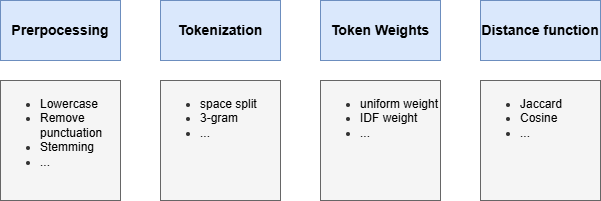
\includegraphics[width=0.7\linewidth]{img/join_configuration.png}
	\end{figure}
\end{frame}



\begin{frame}{Example: Fuzzy Join Distance Score Computation}
	\textbf{Join Function:} $f = (L, SP, EW, JD)$
	\begin{itemize}
		\item \textbf{L}: Lower-casing (Preprocessing)
		\item \textbf{SP}: Space Tokenization
		\item \textbf{EW}: Equal Weights
		\item \textbf{JD}: Jaccard Distance
	\end{itemize}
	
	\vspace{1em}
	\textbf{Inputs:}
	\begin{itemize}
		\item $l = \texttt{"2012 tigers lsu baseball team"}$
		\item $r = \texttt{"2012 lsu baseball team"}$
	\end{itemize}
	
	\vspace{1em}
	\textbf{Tokenization (SP):}
	\begin{itemize}
		\item $l \rightarrow \{2012, tigers, lsu, baseball, team\}$
		\item $r \rightarrow \{2012, lsu, baseball, team\}$
	\end{itemize}
	
	\vspace{1em}
	\textbf{Jaccard Distance:}
	\begin{itemize}
		\item $A \cap B = \{2012, lsu, baseball, team\} \rightarrow |A \cap B| = 4$
		\item $A \cup B = \{2012, tigers, lsu, baseball, team\} \rightarrow |A \cup B| = 5$
		\item $\text{Jaccard Similarity} = \frac{4}{5} = 0.8$
		\item $\text{Jaccard Distance} = 1 - 0.8 = 0.2$
	\end{itemize}
	
	\vspace{1em}
	\textbf{Result:} $f(l, r) = 0.2$
\end{frame}


\begin{frame}{Theoretical foundation: threshold and join configuration}
	
\begin{itemize}
	\item Once the distance $f(l, r)$ is computed:
	\begin{itemize}
		\item It is compared to a threshold\textbf{compared to a threshold} $\theta$  to decide whether to join the string pair $l$ and $r$.
		\item If $f(l, r) \leq \theta$ , the pair is considered \textbf{a match}.
	\end{itemize}
	\item 	Together, the function $f$ and the threshold $\theta$ define what the authors call a \textbf{join configuration}:$$
	C = (f, \theta)
	$$
	\item This configuration encapsulates both:
	\begin{itemize}
		\item How distance is computed.
		\item When two strings are considered similar enough to be joined.
	\end{itemize}
\end{itemize}	

\begin{beamercolorbox}[rounded=true, shadow=true, leftskip=1em, rightskip=1em]{myblock}
	\textbf{Definition:} A join configuration $C$ is a 2-tuple $C = \langle f, \theta \rangle$, where $f \in \mathcal{F}$ is a join function, and $\theta$ is a threshold.\\
	We use $\mathcal{S} = \{ \langle f, \theta \rangle \mid f \in \mathcal{F}, \theta \in \mathbb{R} \}$ to denote the space of join configurations.
\end{beamercolorbox}

\end{frame}


\begin{frame}{Theoretical foundation: fuzzy join mapping}
	Given two tables $L$  and $R$ , a join configuration $C \in \mathcal{S}$ induces a \textbf{fuzzy join mapping} $J_C$ , defined as:
	
	\begin{beamercolorbox}[rounded=true, shadow=true, leftskip=1em, rightskip=1em]{myblock}
	$$
		J_C(r) = \underset{l \in L,\ f(l, r) \leq \theta}{\arg\min} f(l, r),\ \forall r \in R
	$$
	\end{beamercolorbox}
	
	That is
	\begin{itemize}
		\item For each record $r \in R$, find $l \in L$ that minimizes the distance $f(l, r)$, \textbf{only if} that distance is less than or equal to the threshold $\theta$.
		\item If no such $l \in L$ exists such that $f(l, r) \leq \theta$, then $J_C(r)$ is \textbf{empty} — i.e., no match for that record.
	\end{itemize}

\end{frame}


\begin{frame}{Theoretical foundation: the problem with single join configurations}
	
	\begin{columns}
		% Left column: explanation
		\begin{column}{0.52\textwidth}
			Real-world data can exhibit \textbf{multiple types of variations simultaneously}, such as:
			\begin{itemize}
				\item \textbf{Typos}
				\item \textbf{Missing tokens}
				\item \textbf{Extraneous information}
			\end{itemize}
			
			As a result, relying on a \textbf{single join configuration} often fails to capture all valid matches, particularly when high \textbf{recall} is required.
			
			\vspace{0.5em}
			To handle this diversity, the algorithm uses a \textbf{set of join configurations}:
			\[
			U = \{C_1, C_2, \dots, C_K\}
			\]
			
			Instead of relying on a single configuration, the system computes join results from each one.
			
			This approach allows the system to:
			\begin{itemize}
				\item Accommodate diverse types of variations.
				\item Improve overall recall by \textbf{combining multiple perspectives} on similarity.
			\end{itemize}
		\end{column}
		
		
		\begin{column}{0.45\textwidth}
			\centering
			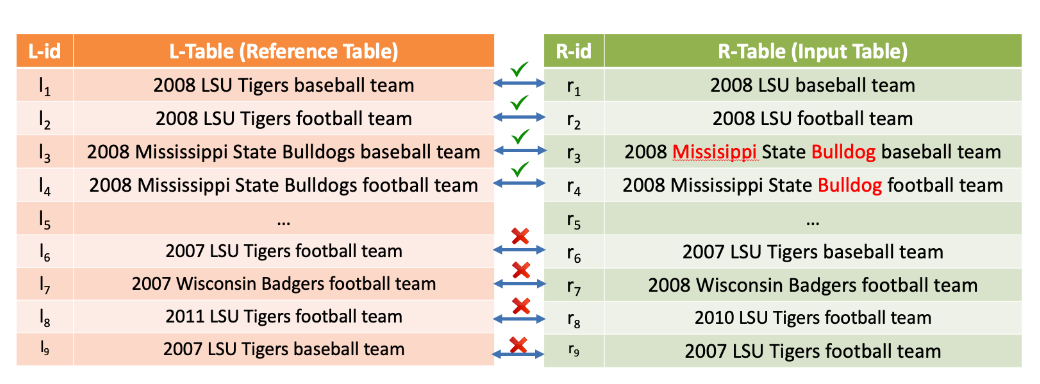
\includegraphics[width=\linewidth]{img/Pasted image 20250331152324.png}
			
			
			\vspace{0.5em}
			\small
			\begin{itemize}
				\item A \textbf{Jaccard distance} with threshold $0.2$ works well for pairs like $(l_1, r_1)$, which differ by only one or two tokens.
				\item However, for pairs like $(l_3, r_3)$ with \textbf{spelling variations}, Jaccard similarity is not enough:
				\begin{itemize}
					\item Jaccard distance $\approx 0.5 \rightarrow$ too high to match under the 0.2 threshold
					\item A more suitable metric is \textbf{Edit Distance}, which can better align such pairs.
				\end{itemize}
			\end{itemize}
		\end{column}

	\end{columns}
	
\end{frame}



\begin{frame}{Theoretical foundation: fuzzy join via multiple configurations}
	
	\begin{itemize}
		\item To handle this diversity, the algorithm uses a \textbf{set of join configurations}:
		\[
		U = \{C_1, C_2, \dots, C_K\}
		\]
		\item Instead of relying on a single configuration, the system computes join results from each.
		\item This approach allows the system to:
		\begin{itemize}
			\item Accommodate diverse types of variations.
			\item Improve overall recall by \textbf{combining multiple perspectives} on similarity.
		\end{itemize}
	\end{itemize}
	
	\vspace{1em}
	
	\begin{beamercolorbox}[rounded=true, shadow=true, leftskip=1em, rightskip=1em]{myblock}
		Given $L$ and $R$, a set of join configurations $U = \{C_1, C_2, \ldots, C_K\}$ induces a \textbf{fuzzy join mapping} $J_U$, defined as:
		\[
		J_U(r) = \bigcup_{C_i \in U} J_{C_i}(r),\ \forall r \in R \tag{2}
		\]
		This means that the overall result of the fuzzy join using configuration set $U$ is the \textbf{union} of results from all individual configurations $C_i \in U$.
	\end{beamercolorbox}
	
	\vspace{0.5em}
	
	Each configuration $C_i \in U$ is designed to capture a \textbf{specific type of string variation} (e.g., typos, missing tokens, extra tokens).
	
	Two records are considered \textbf{joined by the set} $U$ \textbf{if and only if} they are joined by \textbf{at least one} configuration $C_i \in U$.
	
	\begin{itemize}
		\item Each configuration contributes \textbf{high-quality joins} targeted at particular data challenges.
		\item The overall join is more \textbf{robust and comprehensive}.
	\end{itemize}
	

	
\end{frame}

\begin{frame}{Evaluating Join Quality: Precision}
	
	Given two tables $R$ and $L$, and a \textbf{space of join configurations} $\mathcal{S}$, the objective is to find a subset $U \subseteq \mathcal{S}$ that produces \textbf{good fuzzy join results}.
	
	Let:
	\begin{itemize}
		\item $J_U$ be the fuzzy join mapping induced by configuration set $U$
		\item $J_G$ be the \textbf{ground truth} join mapping — the ideal join result
	\end{itemize}
	
	\vspace{0.5em}
	\textbf{Precision} measures how many of the predicted joins are correct:
	
	\[
	\text{precision}(U) =
	\frac{
		\underbrace{|\{ r \in R\ |\ J_U(r) \neq \emptyset,\ J_U(r) = J_G(r) \}|}_{\text{True Positives (TP)}}
	}{
		\underbrace{|\{ r \in R\ |\ J_U(r) \neq \emptyset \}|}_{\text{TP + FP (all predicted joins)}}
	}
	\tag{3}
	\]
	
	\begin{itemize}
		\item \textbf{Numerator (TP)}: Records where a join was predicted and it matched the ground truth.
		\item \textbf{Denominator (TP + FP)}: All records where a join was predicted (correct or not).
	\end{itemize}
	
\end{frame}


\begin{frame}{Evaluating Join Quality: Recall}
	
	\textbf{Recall} measures how many of the correct (ground truth) joins were successfully predicted:
	
	\[
	\text{recall}(U) =
	\underbrace{|\{ r \in R\ |\ J_U(r) \neq \emptyset,\ J_U(r) = J_G(r) \}|}_{\text{True Positives (TP)}}
	\tag{4}
	\]
	
	\begin{itemize}
		\item This is the \textbf{absolute count of True Positives}, i.e., records for which:
		\begin{itemize}
			\item A join was predicted ($J_U(r) \neq \emptyset$), and
			\item It matches the ground truth ($J_U(r) = J_G(r)$)
		\end{itemize}
	\end{itemize}
	
	\vspace{0.5em}
	\textbf{False Negatives (FN)} — cases where a correct join was missed — are defined as:
	\[
	\text{FN} = |\{ r \in R\ |\ J_G(r) \neq \emptyset,\ J_U(r) = \emptyset \}|
	\]
	
	\textit{Note:} The denominator $TP + FN$ is constant across all $U$ for a fixed dataset, so it is omitted in comparisons.
	
\end{frame}


\begin{frame}{Estimating Precision/Recall for a Single Join Configuration}
	
	Given:
	\begin{itemize}
		\item A \textbf{single join configuration} $C = \langle f, \theta \rangle$
		\item Two tables:
		\begin{itemize}
			\item $L$: reference table
			\item $R$: query table
		\end{itemize}
	\end{itemize}
	
	\vspace{0.5em}
	\textbf{Assumption: Complete Reference Table $L$}
	\begin{itemize}
		\item $L$ is assumed to contain \textbf{all possible true matches} for records in $R$.
		\item Ensures that for each $r \in R$, there exists a correct match $l \in L$.
		\item Simplifies analysis by reducing the chance of missing true positives due to an incomplete reference.
	\end{itemize}
	
	\vspace{0.5em}
	\textbf{Geometric View of the Distance Function $f$}
	\begin{itemize}
		\item Join function $f$ embeds records into a \textbf{metric space}.
		\item Records are modeled as points on a \textbf{unit grid}.
		\item Each $l \in L$ is surrounded by \textbf{close variants} (differing by a token, character, etc.).
	\end{itemize}
	
	\vspace{0.5em}
	\setbeamercolor{block title}{bg=blue!10, fg=black}
	\setbeamercolor{block body}{bg=blue!5, fg=black}
	\begin{block}{Analogy: Stars and Planets}
		\begin{itemize}
			\item Reference records $l \in L$ are like \textbf{stars} on a grid.
			\item Query records $r \in R$ are like \textbf{planets} that orbit these stars.
			\item Identifying the best join $J_C(r)$ is like determining \textbf{which star a planet orbits}.
		\end{itemize}
	\end{block}
	
\end{frame}


\begin{frame}{Safe Joins and the Geometry of Fuzzy Matching}
	
	\textbf{Safe Joins with a Complete $L$}
	\begin{itemize}
		\item Define the \textbf{grid width} $w$: typical distance between a record $l$ and its closest neighbors in $L$.
		\item A join is considered \textbf{safe} if the distance $d = f(l, r)$ satisfies:
		\[
		d < \frac{w}{2}
		\]
		\item This guarantees that $r$ lies \textbf{closer to its true match} $l$ than to any other reference point.
	\end{itemize}
	
	\vspace{0.5em}
	\textbf{Why This Matters:}
	\begin{itemize}
		\item Ensures high \textbf{precision} — avoiding false positives caused by ambiguous joins.
		\item Avoids joining $r$ to an incorrect $l'$ that lies at a similar distance.
	\end{itemize}
	
	\vspace{0.5em}
	\textit{Analogy:}
	\begin{itemize}
		\item A planet that lies \textbf{equidistant} between two stars (at $\frac{w}{2}$ each) \textbf{cannot be confidently claimed by either}.
		\item In fuzzy joining, such cases are inherently \textbf{ambiguous} and risky to resolve.
	\end{itemize}
	
\end{frame}



\end{document}
